
\subsection{Embeddings}
Neural networks do not deal well with categorical variables. One hot encoding is a way to handle this. It allows us to represent categorical data as sparse vectors of zeroes and a single 1 representing the specific category. This method has two main drawbacks. Firstly, the dimensionality of the vector representation size grows with the corpus. It can become unmanageable very quick. Secondly, each vector is equidistant from every other vector. This means 'similar' categories are not represented close together in the vector space.

A better way of handling categorical data is through embeddings. When using embeddings we can project categories in a low dimensional latent space and represent them as dense continuous vectors. They are learned parameters and due to this, similar items are projected close together in the latent space. Therefore it is useful in the context of recommendations as we are trying to model user-item similarities. They are also well studied and highly applied in literature for natural language processing to represent words. Embeddings can be pre-trained and adapted to be used in a model or learned end-to-end with the other parameters.

The main inputs to the model consist of user, item and genre embeddings learned iteratively with the rest of the model parameters.

Genres are handled slightly different than the other two because a movie can have more than one genre. The basis of the embedding is multi hot encoding, meaning the vector has a value of one for each category that describes it.

\subsection{Activation function}
In a neural network activation functions are mathematical equations, applied to each neuron, that determine if it should activate or not based on its inputs. This function must be computationally efficient to calculate, differentiable and will generally be non-linear. The last part is very important because without non-linearities a NN would just behave like a single-layer perceptron and would not be able to model complex functions. One exception to this is the output layer for a regression NN which will have a linear activation to allow the prediction of any real value.

Early neural networks were using tanh and sigmoid activation functions. Sigmoid also known as logistic function is S-shaped and bounded by 1 and 0. \ref{eq:sigmoid}
% Simply put an activation function decides if a neuron should `fire`
Traditional sigmoid \ref{eq:sigmoid}, tanh \ref{eq:tanh}

Rectified Linear Unit ReLU \ref{eq:relu}
A major drawback of using ReLU activations is the "dying ReLU" problem.  
leaky ReLU \ref{eq:leakyrelu}
comparison with traditional ones
comparison between relu and leaky relu

\begin{equation}
    \label{eq:sigmoid}
    \begin{aligned}
    f(x) &= \frac{1}{1+e^{-x}} \\
    f'(x) &= f(x)(1 - f(x))
    \end{aligned}
\end{equation}

\begin{equation}
    \label{eq:tanh}
    \begin{aligned}
    f(x) &= \frac{2}{1+e^{-2x}} - 1 \\
    f'(x) &= 1 - f(x)^2
    \end{aligned}
\end{equation}

\begin{equation}
    \label{eq:relu}
    \begin{aligned}
    f(x) &=
    \begin{cases}
        x, & \text{if } x\geq 0 \\
        0, & \text{otherwise}
    \end{cases} \\
    f'(x) &=
    \begin{cases}
        1, & \text{if } x\geq 1 \\
        0, & \text{otherwise}
    \end{cases}
    \end{aligned}
\end{equation}

\begin{equation}
    \label{eq:leakyrelu}
    \begin{aligned}
    f(x) &=
    \begin{cases}
        x, & \text{if } x\geq 0 \\
        0.01x, & \text{otherwise}
    \end{cases} \\
    f'(x) &=
    \begin{cases}
        1, & \text{if } x\geq 1 \\
        0.01, & \text{otherwise}
    \end{cases}
    \end{aligned}
\end{equation}

% \begin{figure}[h!]
%     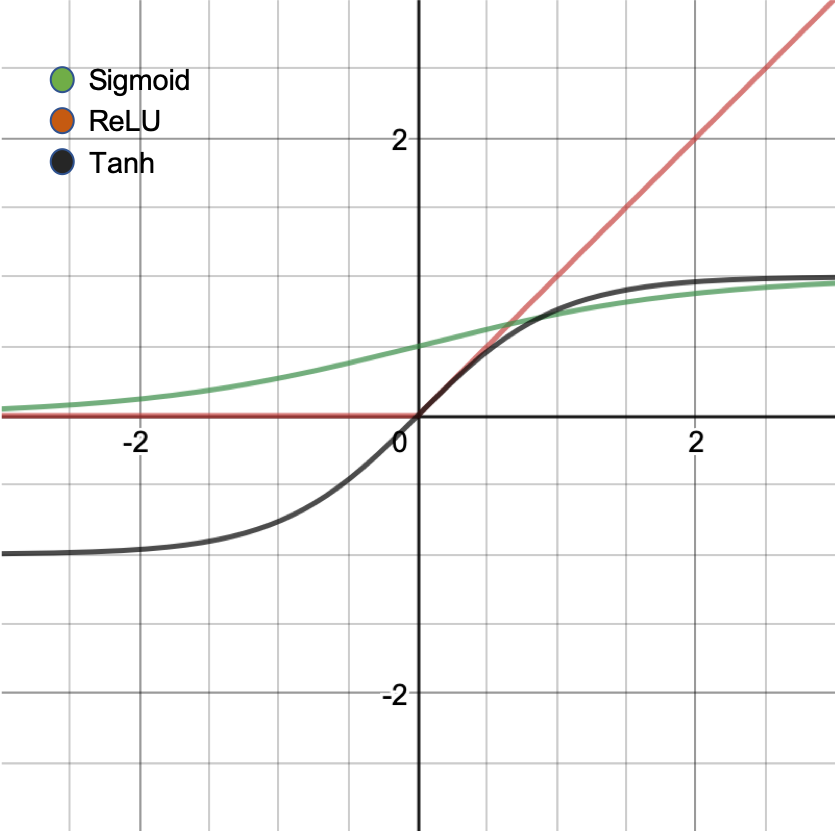
\includegraphics[scale=0.5]{3-activation-func.png}
%     \caption{Activation functions comparison}
% \end{figure}

% \begin{figure}[h!]
%     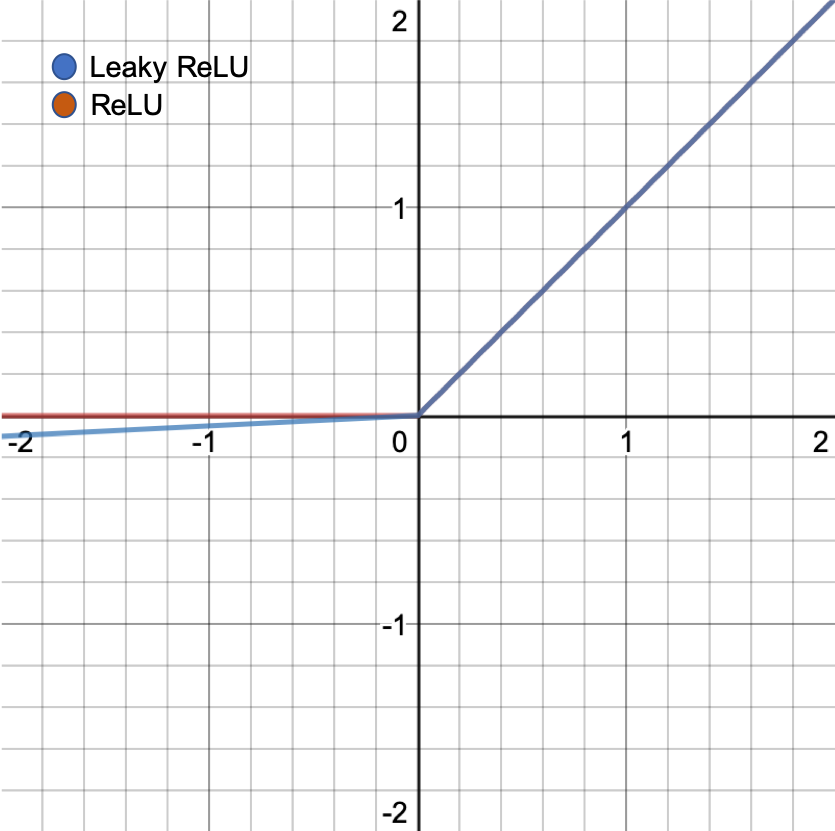
\includegraphics[scale=0.5]{leakyReLUvsReLU.png}
%     \caption{Leaky ReLU vs ReLU}
% \end{figure}

\begin{figure}[h!]
    \subfloat[Activation functions]{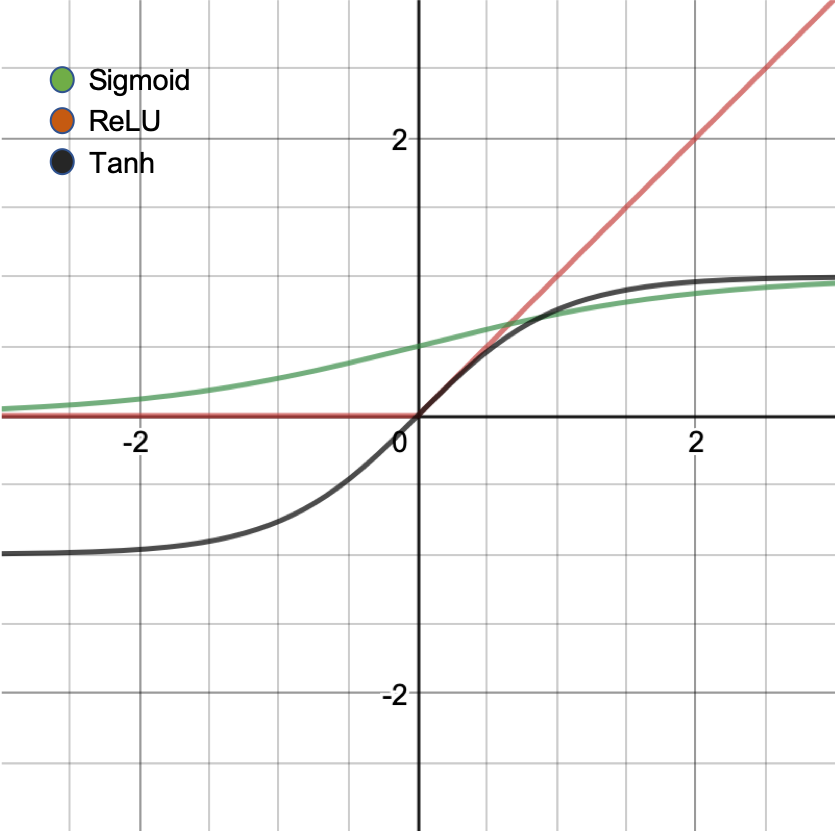
\includegraphics[scale=0.5]{3-activation-func}\label{fig:activations}}
    \hfill
    \subfloat[ReLU vs Leaky ReLU]{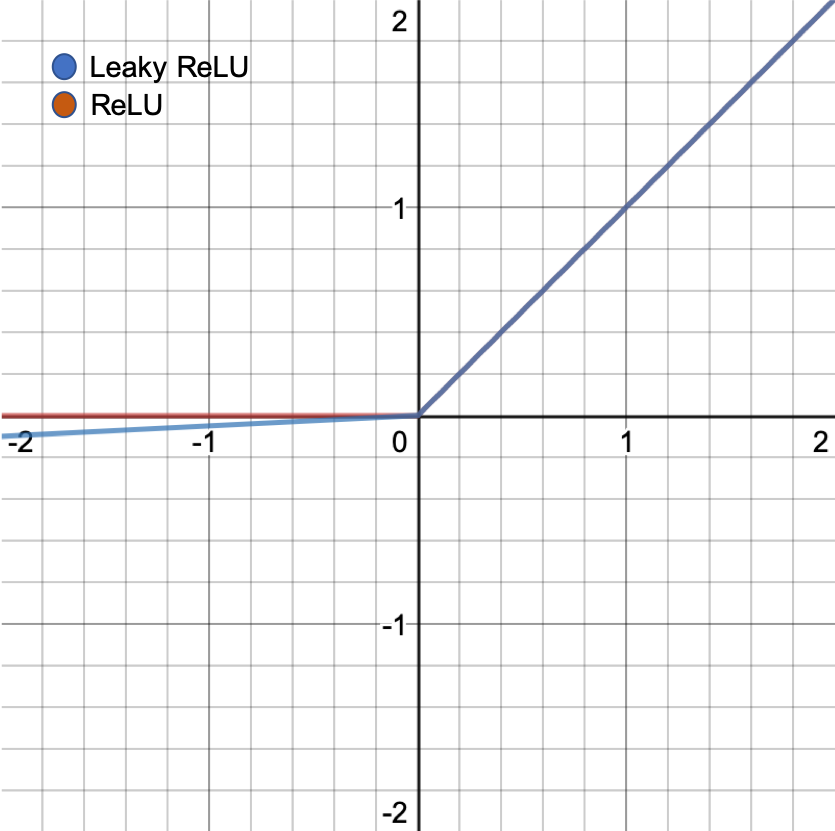
\includegraphics[scale=0.5]{leakyReLUvsReLU}\label{fig:relus}}
\end{figure}


\subsection{Regularization}
One of the most common problems in training neural networks is over-fitting. A model is said to be over-fitting when it performs well on training data but poorly on validation data. Intuitively, it means the model is unable to generalize well and only memorizes the training examples.
This generally occurs if the model is too complex or the size of the training dataset is too small.
Regularization is a method of reducing over-fitting through small modifications of the learning algorithm. The most common types of regularization are l1 and l2. L1 
Kernel Regularization
Activity Regularization
Dropout general value 0.5 gives higher RMSE than 0.2
Batch normalization
% A dropout rate of 0.2 was found to be better and result in a \% decrease in RMSE than the generally used 0.5. 

\subsection{Optimizer}
Optimizers are a very important parameter in NN configuration. Nowadays there is a vast choice of good optimizers. At its core, an optimizer is an iterative method of optimizing for a cost function. At each optimization step, the weights in the NN will be updated based on the negative of the gradient of the cost function. Stochastic gradient descent (SGD) is a variation of gradient descent in that the optimization happens after each training example. In practice, this usually implies mini-batches of between 32 and 1024 data points (\citet{practical_training}). Batch gradient descent involves updating the weights based on the gradient over the whole dataset. SGD optimizes based on an approximation of the gradient, unlike batch gradient descent. This turns out to be useful as it introduces noise in the network which leads to better generalization. It is also more scalable as the whole dataset does not have to be kept in memory. (\citet{practical_training})

% It is well studied and its convergence is mathematically provable. 
\begin{equation}
    \theta = \theta - \alpha \Delta_{\theta} J(\theta ;x^{(i)}y^{(i)})
\end{equation}

More advanced optimizers are built on top of SGD and include things such as adaptive learning rates and momentum to increase convergence speed and overall stability.

One such algorithm is adaptive moment estimation (Adam). Its widely used in literature and converges much faster than SGD. Adam can be seen as a combination of RMSProp and momentum (\citet{Adam}).

Nesterov adaptive moment estimation (NAdam) combines adam with nesterov momentum which improve convergence (cite)

\subsection{Training}
Weight initialization plays an important role in training a neural network. Ideally, we wish the initial weights to be random but not too small and too big, otherwise, it will lead to problems of vanishing or exploding gradients. Xavier normal initialization is one technique that constricts the weights to these characteristics. It works by drawing from a truncated random distribution centered on 0 and with a standard deviation of \(\frac{2}{n_{in} + n_{out}}\), where \(n_{in}\) and \(n_out\) represent the number of inputs and outputs (\citet{initialization}). This is the default initializer used in keras. It is best suited for use in NN that employ tanh activation functions. He normal initialization works better for relu activation. Its similar to xavier, but the standard deviation is \(\frac{2}{n_{in}}\) (\citet{rectifiers}).

\begin{verbatim}
    xavier_w = np.random.rand((n_in, n_out)) * np.sqrt(2 / (n_in + n_out))
    he_w = np.random.rand((n_in, n_out)) * np.sqrt(2 / n_in)
\end{verbatim}

Too speed up the training I have implemented a special generator class extending keras \emph{sequence}. This enables multiprocessing execution of the batch generation algorithm and more importantly it ensures safety and single use of each training example per epoch.
After creating the generator its possible to use the keras \emph{fit\_generator} function with 12 workers and a maximum queue size of 200. These parameters are required in order to enable multi-gpu training and to ensure that the gpus are not idle waiting for data.

\subsection{Architecture}
The NN architecture follows a common tower pattern, where layers near the top are widest and progressively decrease in width. The activation functions employed at the hidden layers are leakyRelu. Each hidden layer is followed by a dropout layer and a batch normalization layer.

\begin{figure}[h!]
    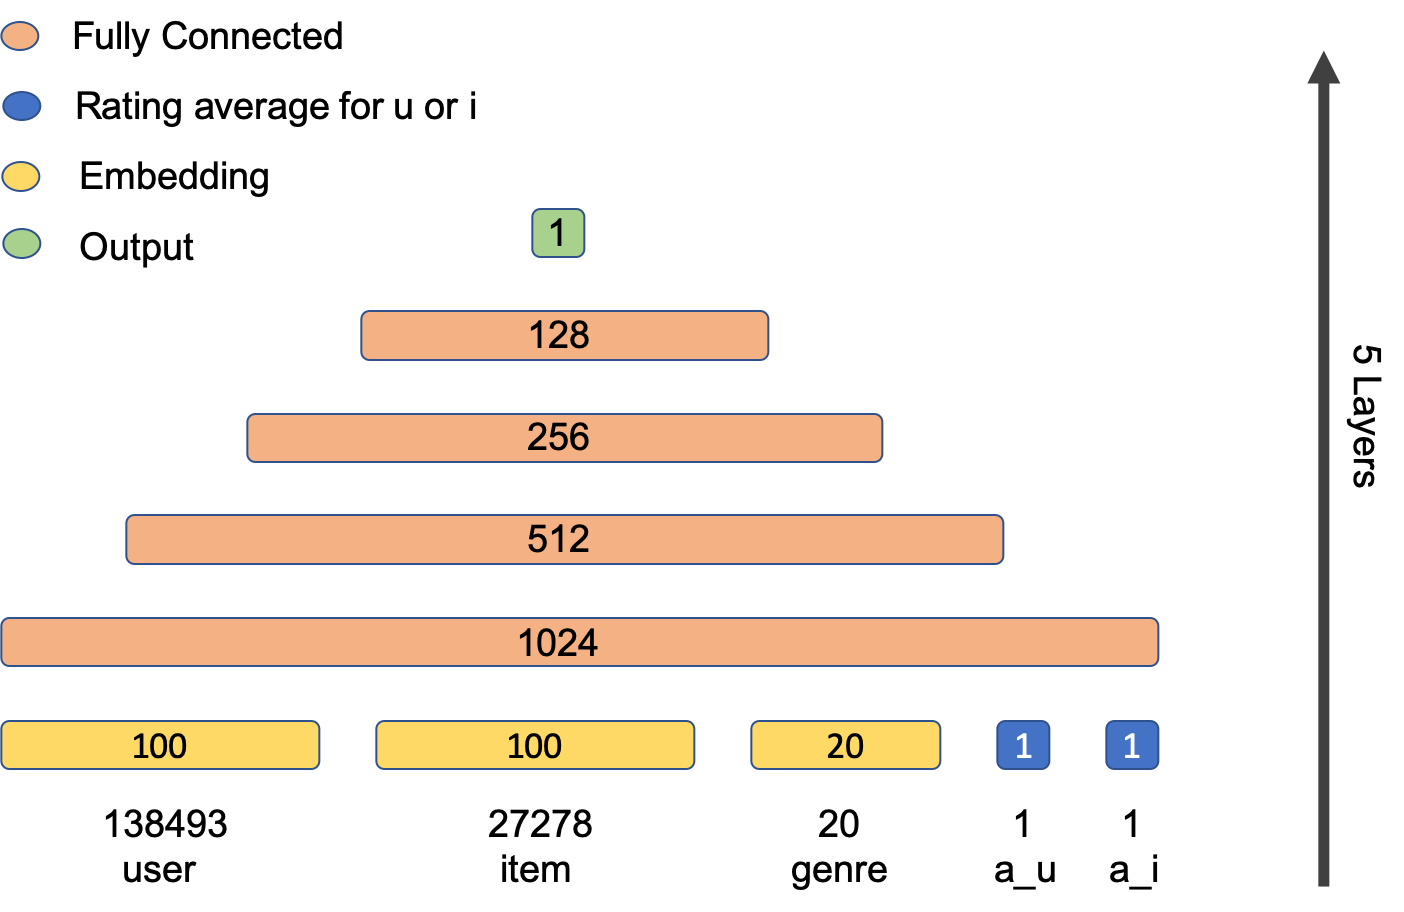
\includegraphics[scale=0.6]{nn_architecture.png}
    \caption{Network architecture}
\end{figure}



\subsection{Serving recommendation \& Api}
Structure of Api.
Create pod that just retrains the model on new ratings. Once finished redeploy pods